\subsubsection{Displaymenu}
\label{subsubsec:Software_Displaymenu}

Das Bedienmenü am Display bietet dem Benutzer viele Freiheiten, was ein umfangreiches und möglichst intuitives Bedienkonzept erforderte. Folgende Einstellungen und Anpassungen können vom Benutzer vorgenommen werden:


\begin{itemize}
\item Getränkeauswahl gemäss Bild oder Listenansicht
\item Zutatenabfrage
\item Bearbeitung von bereits existierenden Cocktails
\item Erstellen neuer Cocktails 
\item Individuelle Zusammenstellung und Positionierung von Flüssigkeiten
\item Zuweisung eines Getränkes zu einem RFID-Tag
\item Anzeige einer Maschineninfo
\item individuelle Beleuchtung der Maschine
\item Maschinen Reinigungsmodus
\end{itemize}

Im folgenden wird auf die gesamte Menüstruktur eingegangen und erklärt, wie diese zu bedienen ist.

\textbf{Hauptansicht}\\
In der Hauptansicht gemäss Abbildung \ref{fig:DisplayHauptmenu} wird die Getränkeauswahl getroffen. Dabei gibt es zwei verschiedene Auswahlmöglichkeiten. Mit den Pfeiltasten nach links oder rechts kann ein Getränk aus der Maschine ausgewählt werden. Es wird dabei immer der Getränkename und eine dazugehörige Abbildung angezeigt, damit dem Kunden der Cocktail auch schmackhaft gemacht werden kann. Will man schneller suchen, so kann man mittels \flqq Liste\frqq~eine Listenansicht öffnen, wobei man mit den Pfeiltasten nach oben und unten scrollen und den gewünschten Cocktail auswählen kann. Wird eine Auswahl getroffen, so gelangt man zurück in die Hauptansicht und der gewählte Cocktail erscheint mit dem dazugehörigen Bild. Mit \flqq Zurück\frqq~gelangt man ebenfalls zurück in die Hautansicht. Es gibt auch Filtermöglichkeiten. Auf der rechten unteren Seite des Display's kann per Klick entschieden werden, ob nur alkoholische, alkoholfreie oder alle Cocktails angezeigt werden. Hat man ein Getränk gefunden und möchte wissen was sich darin befindet und wie viel, so kann man mittels Klick auf \flqq Zutaten\frqq~ein Fenster öffnen, welches einem anzeigt was und wie viel davon sich darin befindet. Möchte man Einstellungen vornehmen, so gelangt man mittels \flqq Menü\frqq~in das Maschinenmenü.

\begin{figure}[H]
	\centering
	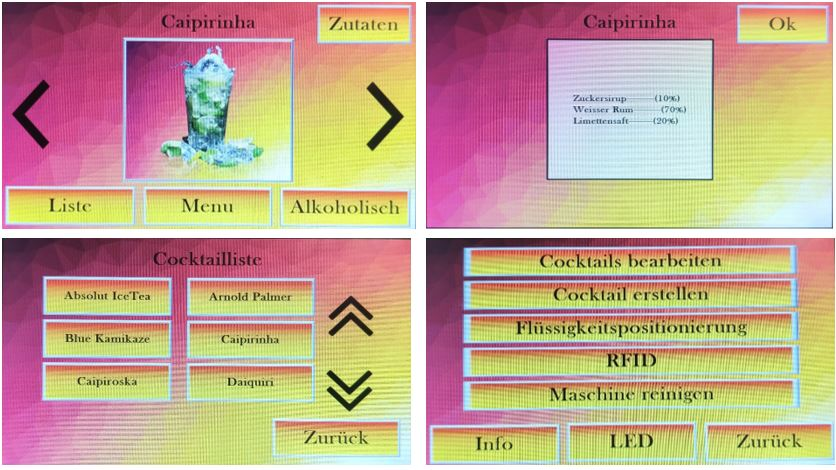
\includegraphics[width=\textwidth]{graphics/DisplayHauptmenu}
	\caption{Hauptansicht der Menüstruktur des Display's \cite{pngimgcom_cocktail_nodate-6}}
	\label{fig:DisplayHauptmenu}
\end{figure}

\textbf{Getränkeauslösung}\\
Wurde die Auswahl für ein Getränk getroffen, so kann man mittels Klick auf das Bild das Getränk auslösen. Dabei gelangt man in eine Abfrage, welche dem Kunden die Wahl lässt, ob er gerne 3dl oder 5dl haben möchte. Mit \flqq Abbrechen\frqq~gelangt man in die Hauptanzeige zurück. Bei Klick auf den entsprechenden Button 3dl oder 5dl wird die gewünschte Grösse des Getränks ausgelöst und am Bildschirm erscheint ein kleiner Text, welcher einem das Warten versüsst. Dazu muss natürlich ein Glas vom Kunden auf den Schlitten gelegt werden. Der Schlitten befördert nun das Glas zu den einzelnen Positionen und füllt es dort ab. Sobald das Getränk fertig ist, fährt der Schlitten an die Ausgangsposition zurück und es wird am Bildschirm angezeigt, dass das Getränk nun fertig ist. Es erscheint danach erneut der Hauptbildschirm und es kann von neuem gestartet werden. Wird während des Erstellungsvorgangs auf \flqq Abbrechen\frqq~gedrückt, so wird der Prozess abgebrochen und das Display zeigt dies an. In Abbildung \ref{fig:DisplayAusloesen} sind die dazugehörigen Bildschirme zu sehen.

\begin{figure}[H]
	\centering
	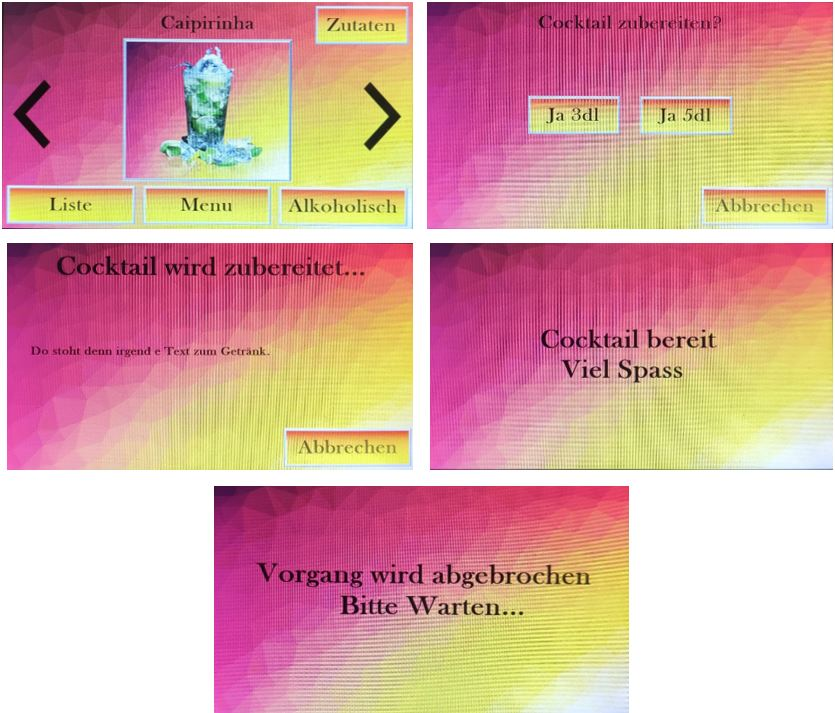
\includegraphics[width=\textwidth]{graphics/DisplayAusloesen}
	\caption{Auslösevorgang der Menüstruktur des Display's \cite{pngimgcom_cocktail_nodate-6}}
	\label{fig:DisplayAusloesen}
\end{figure}

\newpage

\textbf{Maschineninfo und LED-Beleuchtung}\\
Im Maschinenmenü kann unten links eine Info angezeigt werden, welch dem Kunden eine Information gibt, wer diese Maschine gebaut hat und wieso. Die Maschine verfügt über eine eigene Beleuchtung mittels RGBW-LED's. Diese kann vom Kunden individuell eingestellt werden. Klickt man auf \flqq LED\frqq~, so erscheint das Beleuchtungsmenü. in diesem Menü kann die Beleuchtung entweder auf weiss, Rainbow oder Custom eingestellt werden. Wird auf \flqq Weiss\frqq~gedrückt, so leuchtet die Maschine weiss. Bei \flqq Rainbow\frqq~, was standartmässig eingestellt ist, werden die Farben langsam abwechselnd durchgespielt. Wird \flqq Custom\frqq~gedrückt, so können mittel Schieberegler eigene Farben eingestellt werden. Am Anfang stellen sich die Schieberegler auf die zuvor eingestellte Farbe ein. So kann auch mittels Rainbow eine Farbe belassen werden, wenn einem eine Farbe sehr gut gefällt. Wird \flqq Zurück\frqq~betätigt, so gelangt man erneut in das Maschinenmenü. Die dazugehörigen Menübildschirme sind in Abbildung \ref{fig:DisplayInfoLed} zu sehen.

\begin{figure}[H]
	\centering
	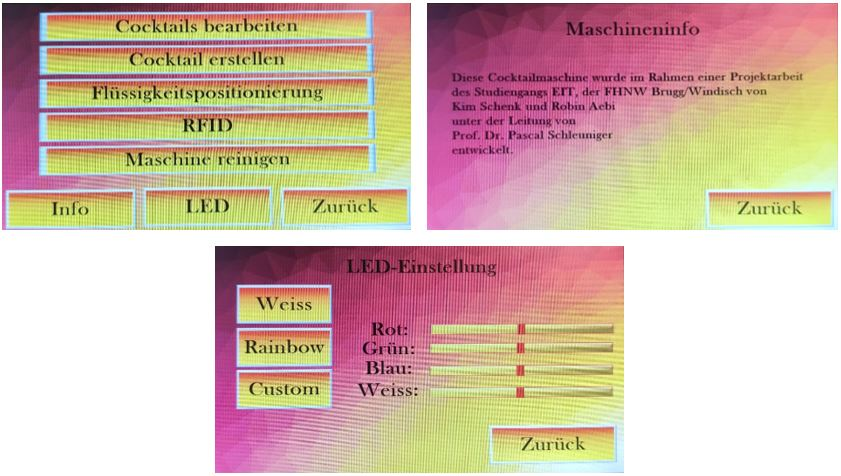
\includegraphics[width=\textwidth]{graphics/DisplayInfoLed}
	\caption{Infomenü und LED Einstellungen der Menüstruktur des Display's}
	\label{fig:DisplayInfoLed}
\end{figure}

\textbf{Cocktails bearbeiten}\\
Um dem Kunden Flexibilität gewährleisten zu können, ist es möglich gemäss Abbildung \ref{fig:DisplayBearbeiten} bereits vorhandene Getränke zu bearbeiten. Somit kann ein Cocktail bei Bedarf hochprozentiger eingestellt werden oder umgekehrt. Um in diesen Bearbeitungsmodus zu gelangen muss \flqq Cocktails bearbeiten\frqq~im Hauptmenü gewählt werden. Es erscheint nun eine Liste, ähnlich der Listenansicht in Abbildung \ref{fig:DisplayHauptmenu}. Hier kann entweder das zu bearbeitende Getränk ausgewählt werden oder mittels \flqq Standarteinst.\frqq~alle Getränke auf den Ursprungszustand gesetzt werden. Mit \flqq Zurück\frqq~gelangt man wieder in das Hauptmenü. Wird ein Getränk ausgewählt, so erscheint eine Liste mit den vorhandenen Flüssigkeiten und einem jeweils dazugehörigen Schieberegler. In diesem Anpassungsmenü sind die momentan eingestellten Dosierungen bereits eingestellt. Diese können nun angepasst werden. Es kann jedoch niemals 100\% über- oder unterschritten werden. Versucht man dies, so kann die Einstellung nicht abgespeichert und es erscheint eine Meldung. Mit \flqq Speichern\frqq~werden die angepassten Einstellungen abgespeichert und es erscheint kurz ein Speicherbildschirm. Danach gelangt man zurück in die Hauptansicht mit dem angepassten Cocktail als Anzeige.

\begin{figure}[H]
	\centering
	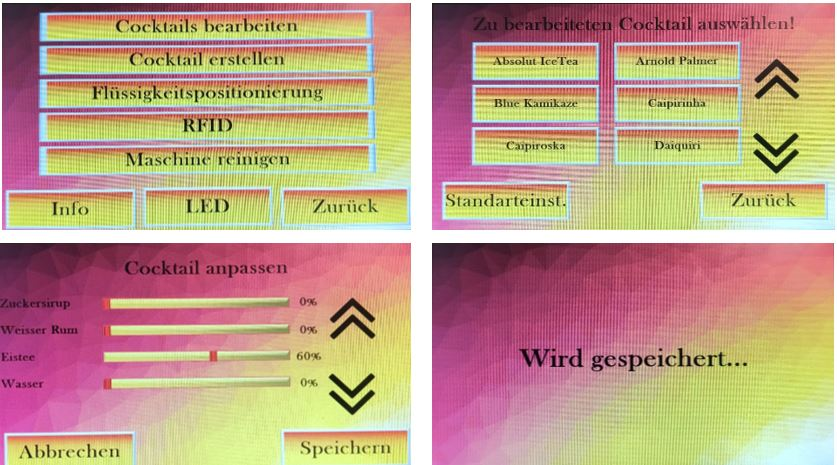
\includegraphics[width=\textwidth]{graphics/DisplayBearbeiten}
	\caption{Cocktail Bearbeitungsmenü der Menüstruktur des Display's}
	\label{fig:DisplayBearbeiten}
\end{figure}

\textbf{Cocktails erstellen}\\
Um dem Kunden noch mehr Flexibilität bieten zu können, ist es auch möglich komplett neue Cocktails zu erstellen gemäss Abbildung \ref{fig:DisplayErstellen}. Dazu muss im Hauptmenü \flqq Cocktail erstellen\frqq~getätigt werden. Man gelangt nun in ein Tastaturmenü, wo man den gewünschten Namen des Cocktails eingeben kann. Dabei kann mit der Taste \flqq Fs\frqq~zwischen Gross- und Kleinschreibweise gewechselt werden. Leuchtet \flqq Fs\frqq~grün, so wird Gross geschrieben und ist \flqq Fs\frqq~schwarz, so wird klein geschrieben. Mit \flqq Del.\frqq~kann ein Zeichen gelöscht und mit Leerzeichen ein Leerzeichen eingesetzt werden. Mit \flqq Abbrechen\frqq~ gelangt man wieder in die Hauptansicht. Mit \flqq OK\frqq~wird der Name zwischengespeichert und man gelangt in eine Listenansicht der vorhandenen Flüssigkeiten, wo gemäss dem Menü in \flqq Cocktails bearbeiten\frqq~die Dosierung eingestellt werden kann.  Auch hier kann 100\% nicht über- oder unterschritten werden. Mit \flqq Speichern\frqq~ wird der Cocktail abgespeichert und man gelangt in die Hauptansicht mit dem eben erstellten Cocktail. Wird \flqq Abbrechen\frqq~betätigt, so gelangt man auch in die Hauptansicht zurück und der Cocktail wird verworfen. Selbst erstellte Cocktails erhalten alle dasselbe Bild in der Hauptansicht. Ausserdem ist es möglich selbst erstellte Cocktails zu löschen. Dazu ist in der Hauptansicht bei den selbst erstellten Cocktails links oben ein Button \flqq Löschen\frqq~zu finden. Wird dieser betätigt, so kommt man in eine Abfrage, welche mit \flqq Ja\frqq~bestätigt und mit \flqq Nein\frqq~dementiert werden kann. 

\begin{figure}[H]
	\centering
	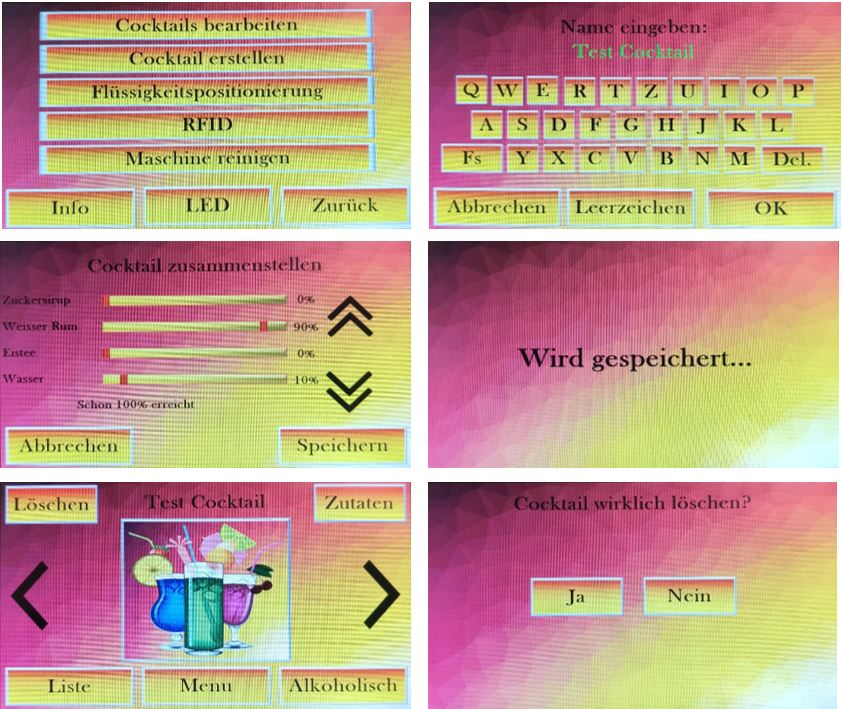
\includegraphics[width=\textwidth]{graphics/DisplayErstellen}
	\caption{Cocktail Erstellungsmenü der Menüstruktur des Display's \cite{noauthor_cocktail_nodate-2}}
	\label{fig:DisplayErstellen}
\end{figure}

\textbf{Flüssigkeitspositionierung}\\
Um dem Kunden absolute Freiheit bei der Bedienung geben zu können, können auch die 12 Flüssigkeiten selbst positioniert und angepasst werden. Wird im Hauptmenü auf \flqq Flüssigkeitspositionierung\frqq~gedrückt, so erscheint eine Zeichnung der Maschine im Grundgerüst, wobei die 12 Flüssigkeitsbehälter zu sehen sind, welche mit Nummern versehen sind. Diese Leuchten grün, wenn eine Flüssigkeit zugewiesen ist. Bei Klick auf eine der 12 Nummern kann die darin enthaltene Flüssigkeit angepasst werden. Es erscheint dabei eine Listenansicht, in welcher die bereits zugewiesene Flüssigkeit grün aufleuchtet. Bei Klick auf eine Zutat aus der Liste wird diese auf der gewählten Position abgespeichert und man gelangt zurück zum Grundgerüst. Im oberen Teil des Bildschirms wird zudem angezeigt, was gerade eingestellt wurde. Wird anstelle einer Flüssigkeit \flqq Keine Flüssigkeit\frqq~gedrückt, so gelangt man zum Grundgerüst zurück und die entsprechende Positionszahl erscheint schwarz. Es ist nun keine Flüssigkeit der Position zugewiesen. Auch diese Änderung wird im Titel angezeigt. Mit \flqq Zurück\frqq~gelangt man wieder ohne Änderung zum Grundgerüst. Die dazugehörigen Bildschirme sind in Abbildung \ref{fig:DisplayPositionierung1} zu sehen. 

\begin{figure}[H]
	\centering
	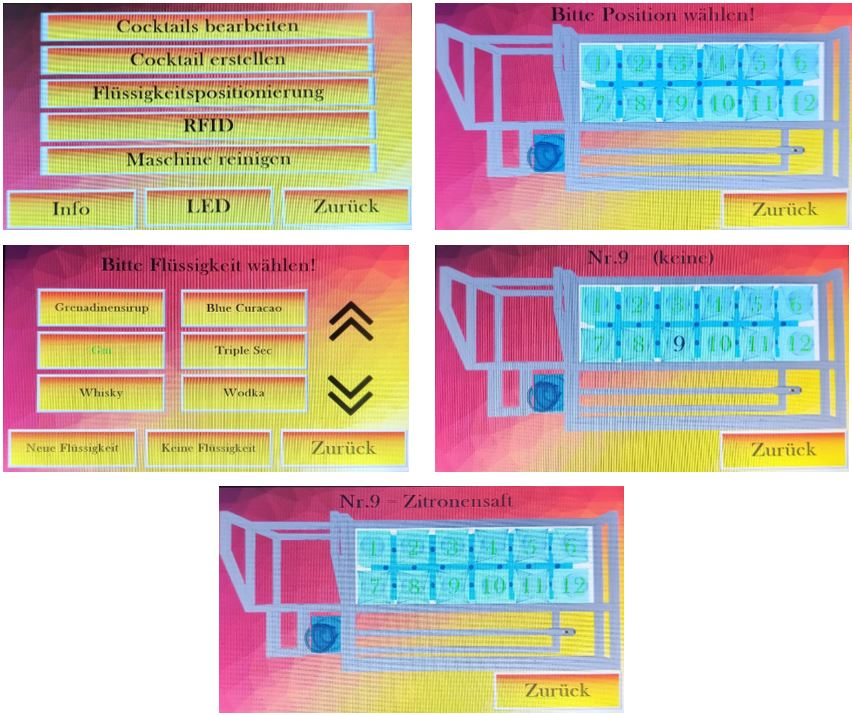
\includegraphics[width=\textwidth]{graphics/DisplayPositionierung1}
	\caption{Flüssigkeitspositionierung der Menüstruktur des Display's}
	\label{fig:DisplayPositionierung1}
\end{figure}

\textbf{Neue Flüssigkeit erstellen und Positionieren}\\
Der Benutzer ist auch bei den Flüssigkeiten nicht auf die vorhandenen Flüssigkeiten reduziert. Auch hier können absolut neue Flüssigkeiten hinzugefügt werden. Dazu kann man bei der Flüssigkeitsauswahl mit dem Button \flqq Neue Flüssigkeit\frqq~eine neue Flüssigkeit erstellen und hinzufügen. Diese Bildschirme sind in Abbildung \ref{fig:DisplayPositionierung2} zu sehen. Wird auf den Button gedrückt, so erscheint erneut eine Tastaturansicht wie bei \flqq Cocktail erstellen\frqq~. Danach kommt eine Abfrage, ob das Getränk kohlensäurehaltig ist. Dies hat den Grund, dass Flüssigkeiten mit Kohlensäure beim Pump- und Messvorgang ihre Kohlensäure verlieren. Flüssigkeiten mit Kohlensäure können erstellt, aber nicht zugewiesen werden. Wird ein Cocktail mit Kohlensäure erstellt, so werden alle Komponenten abgefüllt welche in der Maschine sind und nicht kohlensäurehaltig sind. Nach dem Vorgang wird das Glas zurück gebracht und dem Kunden wird am Display angezeigt, mit welchen kohlensäurehaltigen Flüssigkeiten und mit wie viel davon der Cocktail extern aufgefüllt werden muss. Nach der Abfrage der Kohlensäure kommt eine weitere Abfrage, ob die Flüssigkeit Alkohol enthält. Dies ist wichtig für den Filter in der Hauptanzeige rechts unten. Nach dieser Abfrage wird die Flüssigkeit eingelesen und erstellt. Es wird auch eine  neue Cocktailliste erstellt, denn es werden dem Kunden jeweils nur die Cocktails angezeigt, welche mit den abgespeicherten Flüssigkeiten auch wirklich machbar sind. Die anderen bereits erstellten Cocktails bleiben gespeichert, werden jedoch ausgeblendet. Das Selbe geschieht auch, wenn man beim Grundgerüst auf \flqq Zurück\frqq~drückt. Die Änderungen werden übernommen und eine neue Cocktailliste wird erstellt.

\begin{figure}[H]
	\centering
	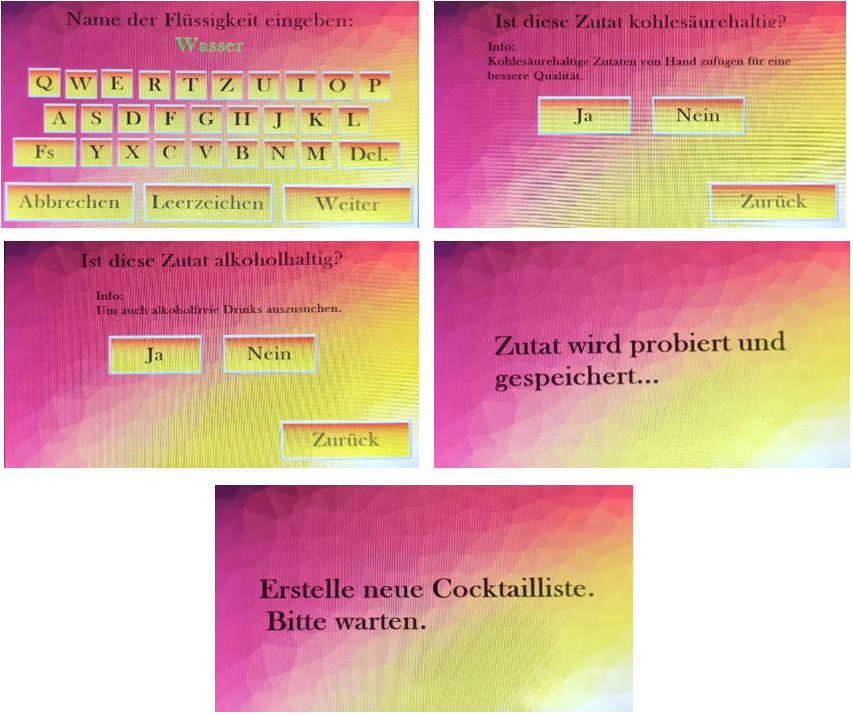
\includegraphics[width=\textwidth]{graphics/DisplayPositionierung2}
	\caption{Flüssigkeitserstellung der Menüstruktur des Display's}
	\label{fig:DisplayPositionierung2}
\end{figure}

\textbf{RFID-Zuweisung}\\
Im Hauptmenü können auch die RFID-Tag's zugewiesen werden. Dabei muss der Button \flqq RFID\frqq~\newline gedrückt werden. Wird dies gemacht, so erscheint eine Liste mit den 10 Tag-Nummern. Mit den Pfeiltasten kann nach unten oder oben gescrollt werden. Mit \flqq Zurück\frqq~gelangt man erneut in das Hauptmenü. Bei Klick auf eine Nummer erscheint die Cocktailliste, wobei ein Getränk ausgewählt werden kann, welches dem vorherig ausgewählten Tag zugewiesen werden soll. Wir ein Getränk ausgewählt, so wird dieses auf dem Tag abgespeichert und man gelangt zur Hauptansicht. Mit \flqq Zurück\frqq~gelangt man erneut zu der Tag-Nummer-Liste. Die dazugehörigen Bildschirme sind in Abbildung \ref{fig:DisplayRFID} zu sehen. 

\begin{figure}[H]
	\centering
	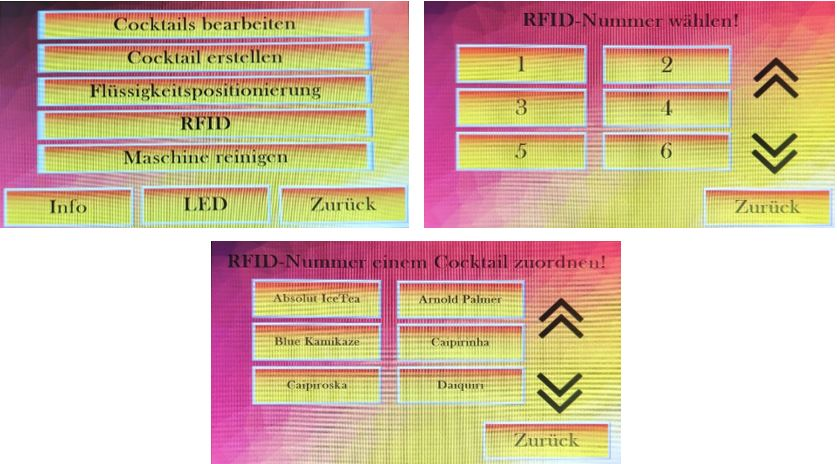
\includegraphics[width=\textwidth]{graphics/DisplayRFID}
	\caption{RFID-Zuweisung der Menüstruktur des Display's}
	\label{fig:DisplayRFID}
\end{figure}

\textbf{Maschinenreinigung}\\
Um ein Verkleben der Schläuche und Pumpen nach der Party zu verhindern, wurde ein Reinigungsvorgang abgespeichert. Dazu kann im Hauptmenü \flqq Maschine reinigen\frqq~gewählt werden. Man wird dabei durch einen Reinigungungsvorgang geführt gemäss den Bildschirmen in Abbildung \ref{fig:DisplayReinigen}.

\begin{figure}[H]
	\centering
	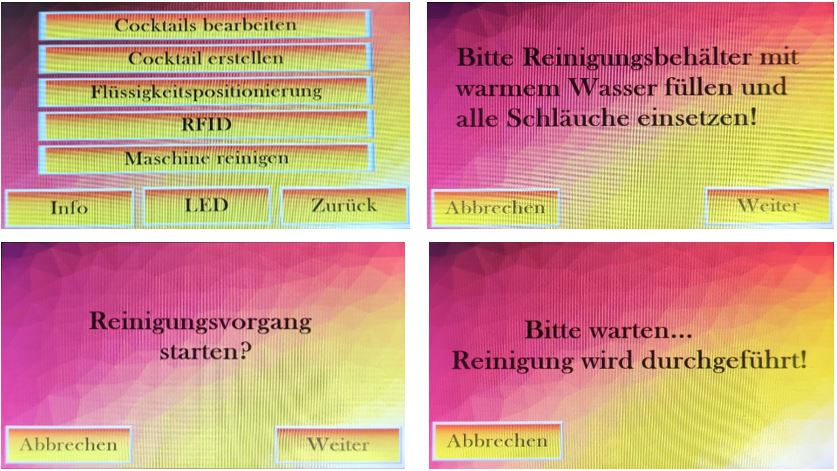
\includegraphics[width=\textwidth]{graphics/DisplayReinigen}
	\caption{Reinigungsmodus der Menüstruktur des Display's}
	\label{fig:DisplayReinigen}
\end{figure}

\newpage


